%%%%%%%%%%%%%%%%%%%%%%%%%%%%%%%%%%%%%%%%%%%%%%%%%%%%
%    Canadian AI Latex Template    %
%%%%%%%%%%%%%%%%%%%%%%%%%%%%%%%%%%%%%%%%%%%%%%%%%%%%
\documentclass[10pt]{cai}

\begin{document}
% Editorial staff will replace the following values:
% 1. Conference Year
% 2. Issue number
% 3. Article DOI
\def\conferenceyear{2025}
\volumeheader{38}{0}%{00.000}
\begin{center}

\title{Development of a Reinforcement Learning Enabled Cattle Tracker Prototype}
\maketitle

\thispagestyle{empty}

% Add Authors and Affiliations in the camera ready
% for the double blind review, please leave this section as is 
\begin{tabular}{cc}
First Author\upstairs{\affilone,*}, Second Author\upstairs{\affilone}, Third Author\upstairs{\affilthree}
\\[0.25ex]
{\small \upstairs{\affilone} Affiliation One} \\
{\small \upstairs{\affiltwo} Affiliation Two} \\
{\small \upstairs{\affilthree} Affiliation Three} \\
\end{tabular}
  
% Replace with corresponding author email address
\emails{
  \upstairs{*}corresponding\_author@example.ca 
}
\vspace*{0.2in}
\end{center}

\begin{abstract}
This is just a sample \LaTeX template. As usual, most of the customization for the proceedings is done in the \texttt{cai.cls} file. 
\end{abstract}

% add your keywords
\begin{keywords}{Keywords:}
Internet of Things (IoT), reinforcement learning.
\end{keywords}
\copyrightnotice

\section{Introduction}

There is an estimated 1.5 million beef cows in Alberta with a portion of those being free-range cattle who are allowed to graze on large pastures for extended periods of time.
Many farmers and researchers are interested in tracking movement of these cattle to asess the health of the herd, and to monitor the location of the cattle.
These trackers take the form of collars, or ear tags and are equipped with sensors, batteries, and communication modules.
The installation of the trackers is often a time consuming process so a tracker is expected to operate for extended periods of time (months) without human intervention.
Given the size of the devices and the environment that they are expected to operate in, there is a limited amount of power budget available to the device and it beocmes a balancing act to ensure contiunuous operation, transmission and data collection.
Reasearchers would like a device that transmits information at high rates as higher fidelity information allows them to make better conclusions about the state of the herd.

The paradigm of Internet of Things (IoT) devices has emerged over the last two decade as a way to deploy compute and intelligence throughout the environment.
% The number of IoT devices is expected to grow to 75 billion by 2025 \cite{gubbiInternetThingsIoT2013}.
The devices are often small, low power, and have limited communication capabilities, but provide insights into the environment that they are deployed in.
The cattle trackers are an example of an IoT device that is deployed in the environment to provide insights into the health and location of the herd.
IoT devices combine sensors, communication modules, storage, and compute to provide insights into the environment that they are deployed in.
IoT devices come as networks or individual devices and in the case of a cattle tracker, ideally a tracker would be self-sufficient as a stand-alone item.
With the spread of the internet and Starlink-like services, it is possible to have a tracker that is connected to the internet and can send data to the cloud, which enables the farmer to monitor the herd from anywhere in the world.
Again we have the challenge of limited power budget and the need to transmit data at high rates.
The power budget can be extended with the use of solar power. 
Solar power is susceptible to weather conditions and the amount of sunlight that is available to the device, which in the case of cattle trackers also depends on the location/orientation of the cattle.

Reinforcement learning is a branch of machine learning that is allows an agent to learn optimum actions to take in an environment to maximize a reward.
The agent learns these actions by interacting with the environment and receiving feedback on the actions that it takes.
Reinforcement learning has been used in a variety of applications such as playing games, optimizing energy consumption, and optimizing the operation of IoT devices.
Machine learning deployed on IoT devices is somtimes referred to as TinyML or AIoT [Check this, since this is Copilot generated text].
On one hand the addition of intelligence to the device allows it to make better decisions, but on the other hand the addition of intelligence to the device increases the power consumption of the device.
Q-learning is a reinforcement learning algorithm that is used to optimize the actions that an agent takes in an environment and has been used in a variety of applications such as optimizing the operation of IoT devices.

In this paper we propose a reinforcement learning enabled cattle tracker prototype that is able to optimize the energy consumption of the cattle tracker.
The cattle tracker alternates between sleeping to conserve power and decision making. 
It is faced with three decision points: 

\begin{itemize}
  \item when to transmit data (high power consumption)
  \item when to collect and store data (medium power consumption)
  \item when to do nothing instead (lowest power consumption)
\end{itemize}

Data transmission is needed to check in and ensure that the device and the cattle is still operational, but consumes a large amount of power.
Data collection and storage is needed to ensure uninterrupted data collection, and consumes a medium amount of power.
Doing nothing consumes the least amount of power, but the device incurs gaps in the data collection, which should only be done to avoid draining the battery to an empty state.
Doing nothing will get the device through the night/day to ensure that it doesn't end up in a weird state by discharging the battery completely.

\section{Related Work}

IoT Sensors are organized as follows:
\begin{itemize}

\item Edge devices are the sensors that collect data.
\item Fog layer which include edge computing devices and IoT gateways.
\item Cloud layer which includes the cloud servers.
\end{itemize}

The challenges of IoT sensors are \cite{chenDeepReinforcementLearning2021}:

- limited battery life

- limited processing power

- limited storage


IoT Networks have been used in a variety of applications

- In \cite{hribarUsingDeepQLearning2019} the authors use deep Q-learning to extend the life of generic sensors networks with non-rechargable batteries by monitoring and optimizing a network of sensors.

- In \cite{yamsaniIoTBasedLivestockMonitoring2024} the authors use IoT networks to monitor the health of livestock across the physical, network, edge and cloud layers.

Contrary to the above works, we propose a single sensor agent, that decides when to transmit, collect and store, or send data to the cloud. This is done by using reinforcement learning to optimize the energy consumption of the sensor.

\section{System Design and Architecture}

\section{Implementation}

\section{Results}

The developed reinforcement learning-enabled cattle tracker prototype was successfully assembled and tested. The prototype consists of key components such as a solar panel, battery, communication module, and processing unit, as shown in Figure~\ref{fig:prototype}.

\begin{figure}[htbp]
  \centering
  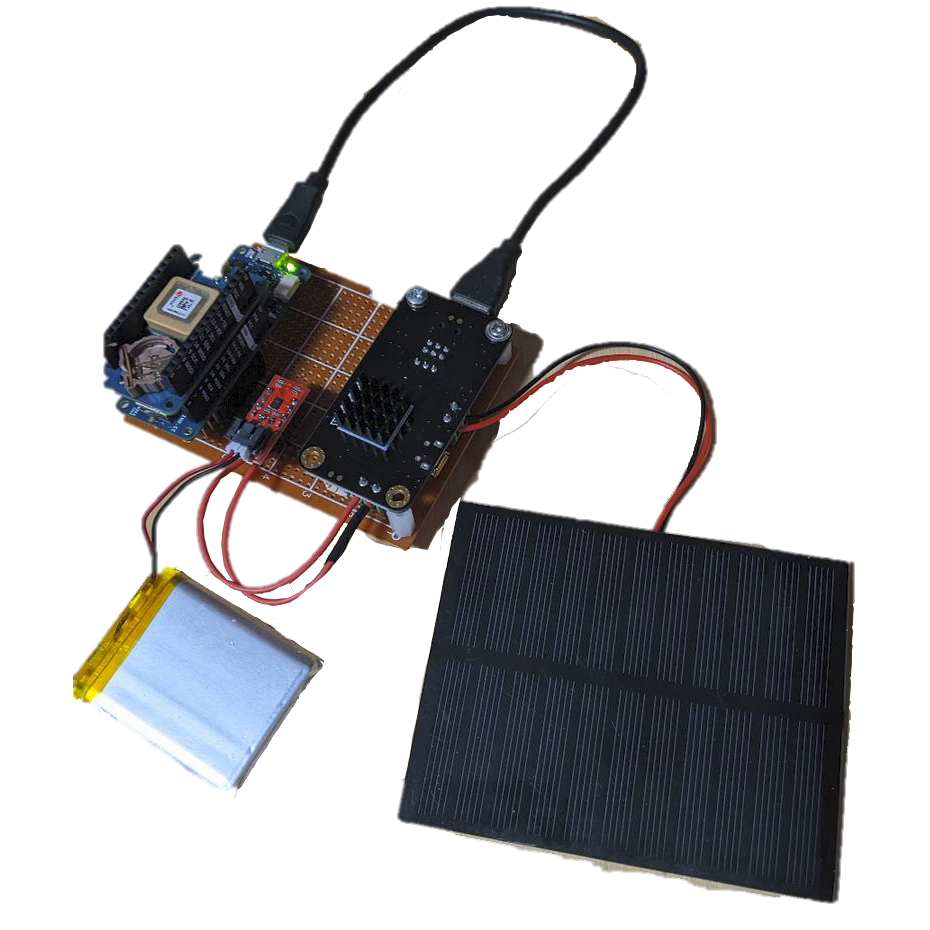
\includegraphics[width=0.5\textwidth]{./figs/prototype_clean.png}
  \caption{Prototype of the reinforcement learning-enabled cattle tracker. The device consists of a solar panel for power harvesting, a rechargeable battery, and an embedded microcontroller for decision-making and communication.}
  \label{fig:prototype}
\end{figure}

The system was evaluated based on its power consumption, data transmission efficiency, and overall performance in real-world conditions. The reinforcement learning algorithm optimized the power usage by balancing data collection, storage, and transmission to ensure continuous operation.

Additionally, the power levels of the device over time were analyzed to assess energy efficiency. Figure~\ref{fig:power_levels} shows the variation in power consumption during different operational phases.

\begin{figure}[htbp]
    \centering
    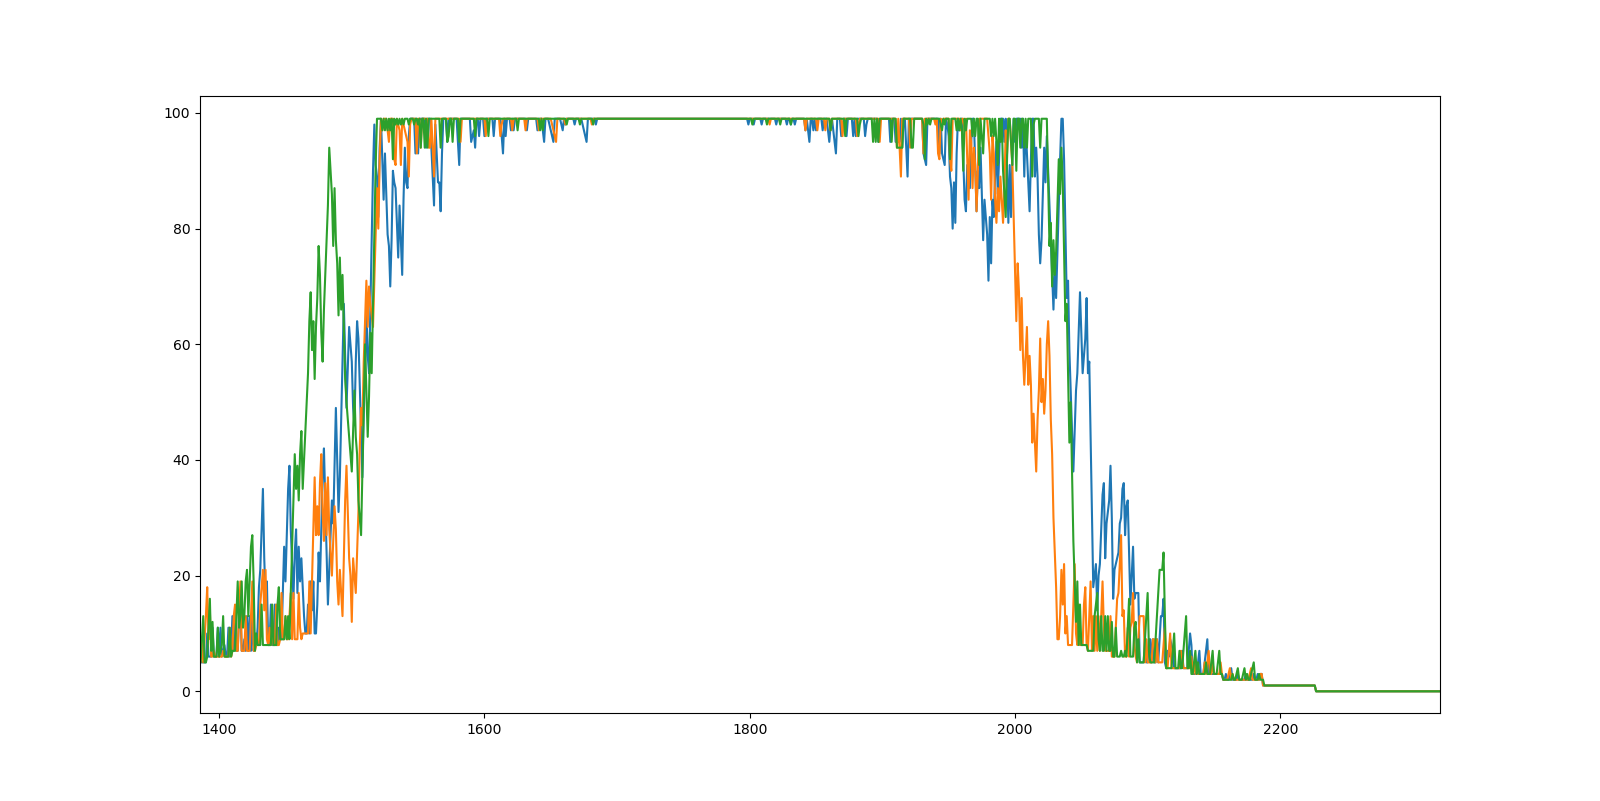
\includegraphics[width=0.8\textwidth]{./figs/power_levels.png}
    \caption{Power consumption levels of the cattle tracker over time. Different colors represent different operational phases such as data transmission, storage, and idle states.}
    \label{fig:power_levels}
\end{figure}


\section{Conclusion}


\section*{Acknowledgements}
We would like to acknowledege the funding provided by NeurAlbertaTech for this project.

%Appendixes go here
\appendix

\section{Example of math equation }
%\label{appendix-customize-this-label}
Binomial theorem: \cite{hribarUsingDeepQLearning2019}
\begin{equation}
(x+y)^n=\sum_{\substack{k=0}}^{n}\dbinom{n}{k}x^{n-k}y^k
\end{equation}


% All references should be stored in the file "references.bib".
% That call to use that file is in "cai.cls". 
% Please do not modify anything below this line.
\printbibliography[heading=subbibintoc]

\end{document}
